\documentclass[twoside]{book}

% Packages required by doxygen
\usepackage{fixltx2e}
\usepackage{calc}
\usepackage{doxygen}
\usepackage[export]{adjustbox} % also loads graphicx
\usepackage{graphicx}
\usepackage[utf8]{inputenc}
\usepackage{makeidx}
\usepackage{multicol}
\usepackage{multirow}
\PassOptionsToPackage{warn}{textcomp}
\usepackage{textcomp}
\usepackage[nointegrals]{wasysym}
\usepackage[table]{xcolor}

% Font selection
\usepackage[T1]{fontenc}
\usepackage[scaled=.90]{helvet}
\usepackage{courier}
\usepackage{amssymb}
\usepackage{sectsty}
\renewcommand{\familydefault}{\sfdefault}
\allsectionsfont{%
  \fontseries{bc}\selectfont%
  \color{darkgray}%
}
\renewcommand{\DoxyLabelFont}{%
  \fontseries{bc}\selectfont%
  \color{darkgray}%
}
\newcommand{\+}{\discretionary{\mbox{\scriptsize$\hookleftarrow$}}{}{}}

% Page & text layout
\usepackage{geometry}
\geometry{%
  a4paper,%
  top=2.5cm,%
  bottom=2.5cm,%
  left=2.5cm,%
  right=2.5cm%
}
\tolerance=750
\hfuzz=15pt
\hbadness=750
\setlength{\emergencystretch}{15pt}
\setlength{\parindent}{0cm}
\setlength{\parskip}{3ex plus 2ex minus 2ex}
\makeatletter
\renewcommand{\paragraph}{%
  \@startsection{paragraph}{4}{0ex}{-1.0ex}{1.0ex}{%
    \normalfont\normalsize\bfseries\SS@parafont%
  }%
}
\renewcommand{\subparagraph}{%
  \@startsection{subparagraph}{5}{0ex}{-1.0ex}{1.0ex}{%
    \normalfont\normalsize\bfseries\SS@subparafont%
  }%
}
\makeatother

% Headers & footers
\usepackage{fancyhdr}
\pagestyle{fancyplain}
\fancyhead[LE]{\fancyplain{}{\bfseries\thepage}}
\fancyhead[CE]{\fancyplain{}{}}
\fancyhead[RE]{\fancyplain{}{\bfseries\leftmark}}
\fancyhead[LO]{\fancyplain{}{\bfseries\rightmark}}
\fancyhead[CO]{\fancyplain{}{}}
\fancyhead[RO]{\fancyplain{}{\bfseries\thepage}}
\fancyfoot[LE]{\fancyplain{}{}}
\fancyfoot[CE]{\fancyplain{}{}}
\fancyfoot[RE]{\fancyplain{}{\bfseries\scriptsize Generated by Doxygen }}
\fancyfoot[LO]{\fancyplain{}{\bfseries\scriptsize Generated by Doxygen }}
\fancyfoot[CO]{\fancyplain{}{}}
\fancyfoot[RO]{\fancyplain{}{}}
\renewcommand{\footrulewidth}{0.4pt}
\renewcommand{\chaptermark}[1]{%
  \markboth{#1}{}%
}
\renewcommand{\sectionmark}[1]{%
  \markright{\thesection\ #1}%
}

% Indices & bibliography
\usepackage{natbib}
\usepackage[titles]{tocloft}
\setcounter{tocdepth}{3}
\setcounter{secnumdepth}{5}
\makeindex

% Hyperlinks (required, but should be loaded last)
\usepackage{ifpdf}
\ifpdf
  \usepackage[pdftex,pagebackref=true]{hyperref}
\else
  \usepackage[ps2pdf,pagebackref=true]{hyperref}
\fi
\hypersetup{%
  colorlinks=true,%
  linkcolor=blue,%
  citecolor=blue,%
  unicode%
}

% Custom commands
\newcommand{\clearemptydoublepage}{%
  \newpage{\pagestyle{empty}\cleardoublepage}%
}

\usepackage{caption}
\captionsetup{labelsep=space,justification=centering,font={bf},singlelinecheck=off,skip=4pt,position=top}

%===== C O N T E N T S =====

\begin{document}

% Titlepage & ToC
\hypersetup{pageanchor=false,
             bookmarksnumbered=true,
             pdfencoding=unicode
            }
\pagenumbering{alph}
\begin{titlepage}
\vspace*{7cm}
\begin{center}%
{\Large General 6-\/\+R\+\_\+\+Inverse Kinematics \\[1ex]\large v1 }\\
\vspace*{1cm}
{\large Generated by Doxygen 1.8.13}\\
\end{center}
\end{titlepage}
\clearemptydoublepage
\pagenumbering{roman}
\tableofcontents
\clearemptydoublepage
\pagenumbering{arabic}
\hypersetup{pageanchor=true}

%--- Begin generated contents ---
\chapter{Description}
\label{index}\hypertarget{index}{}This file documents the use of the function \textquotesingle{}Inverse\+Kinematics\+General6R\textquotesingle{}, to compute the inverse kinematics solutions of general 6-\/R serial manipulator, along with its dependencies. The function can be located in the \textquotesingle{}IK\textquotesingle{} folder and its usage has been demonstrated through three examples, situated in the folders \textquotesingle{}example1\textquotesingle{}, \textquotesingle{}example2\textquotesingle{}, and \textquotesingle{}example3\+\_\+\+Jaco\textquotesingle{}. In the folder \textquotesingle{}example1\textquotesingle{}, the numerical example taken by \textquotesingle{}Raghavan and Roth\textquotesingle{} in their 1990 paper on this topic has been implemented, in the folder \textquotesingle{}example2\textquotesingle{}, the numerical example taken by \textquotesingle{}Liu and Zhu\textquotesingle{} in their 2007 paper has been implemented, and in the folder \textquotesingle{}example3\+\_\+\+Jaco\textquotesingle{},the inverse kinematics algorithm has been implemented on the general 6-\/R robot, Jaco.\hypertarget{index_input}{}\section{Input files and other dependencies\+:}\label{index_input}
\begin{DoxyVerb}The inputs to the function 'InverseKinematicsGeneral6R' are the D-H parameters of the robot and its End-effector pose, which have been denoted by 'dhmat' and 'eemat'
in the function. The inputs 'dhmat' and 'eemat' are being taken from separate 'CSV' files. For the input 'dhmat', the corresponding 'CSV' file should 
have 3 rows and 6 columns, with the '1st' row representing the D-H parameter 'a' of the robot, with the six column entries of that row representing the 
values of 'a1' to 'a6' for the robot. The values of 'a1' to 'a6' should be in meters. The 2nd row represents the D-H parameter 'alpha' of the robot with 
the six column entries of that row representing the values of 'alpha1' to 'alpha6' for the robot. The values of 'alpha1' to 'alpha6' should be in radians. 
The 3rd row represents the D-H parameter 'd' of the robot with the six column entries of that row representing the values of 'd1' to 'd6' for the robot.
The values of 'd1' to 'd6' should be in meters. In this algorithm, the robots have been modelled using the classic D-H parameters. 
So, if the robot has been modelled using modified D-H parameters, then that must be converted into classic D-H parameters, which can then be used as input 
to the 'CSV' file in the way described above to create the 'dhmat'. In the folder 'example1', one such CSV file can be located named, 'dhmat_Raghavan_Roth.csv'.
Similar files are there in the other example folders as well.

For the other input 'eemat' to the function 'InverseKinematicsGeneral6R', the corresponding 'CSV' file should have 4 rows and 3 columns, the 1st row of which represents
the 1st column of the rotation matrix, representing the orientation of the end-effector  of the robot w.r.t the base frame. The 2nd row of this 'CSV' file
represents the 2nd column of the aforementioned rotation matrix, the 3rd row of the 'CSV' file represents the 3rd column of the aforementioned rotation matrix 
and the 4th row of the 'CSV' file represents the position vector (Px, Py, Pz) of the end-effector w.r.t. base frame, and values of the entries of the 
position vector should also be in meters. In the folder 'example1', one such 'CSV' file can be located named, 'eemat_Raghavan_Roth.csv'. Similar files are there 
in the other example folders as well.

Following the 1990 paper by Raghavan and Roth and 1992 paper by Manocha and Canny on Inverse kinematics of general 6-R robots, 
one can arrive at the 12 x 12 matrix, whose entries are quadratic polynomial in x3, lets call it 'capsigdd'. When the problem 
of root finding of the determinant of the matrix, capsigdd, is reduced to an eigenvalue problem, the matrix capsigdd can further 
be decomposed into (A * x3^2 + B * x3 + C), where A, B and C are 12 x 12 matrices and x3 = tan(theta3 / 2). In the function 'InverseKinematicsGeneral6R', 'A', 'B', and 'C' 
is represented by cmatx2, cmatx1, and cmatx0 repectively, each of the entries of which are functions of the D-H parameters and the End-effector pose.  
The 12 x 12 coefficient matrices 'cmatx0', 'cmatx1', and 'cmatx2' in the function 'InverseKinematicsGeneral6R' has been formed by calling functions from the folders 
Coeff_x0, Coeff_x1, and Coeff_x2 respectively. Each of the files in these folders has been formed out of the expressions generated in CAS Mathematica,
after simplifying the entries of the corresponding coefficient matrices.
\end{DoxyVerb}
\hypertarget{index_output}{}\section{Output files\+:}\label{index_output}
\begin{DoxyVerb}The output file is also a 'CSV' file, in which the all the solutions to the inverse kinematics problem for the general 6-R serial manipulator in consideration,
are stored. In the folder 'example1', one such 'CSV' file can be located named, 'example1_output.csv'. Similar files are there in the other example folders as well.\end{DoxyVerb}
 
\chapter{Data Structure Index}
\section{Data Structures}
Here are the data structures with brief descriptions\+:\begin{DoxyCompactList}
\item\contentsline{section}{\hyperlink{struct_csv_parser}{Csv\+Parser} }{\pageref{struct_csv_parser}}{}
\item\contentsline{section}{\hyperlink{struct_csv_row}{Csv\+Row} }{\pageref{struct_csv_row}}{}
\item\contentsline{section}{\hyperlink{struct_residue}{Residue} }{\pageref{struct_residue}}{}
\item\contentsline{section}{\hyperlink{struct_solution}{Solution} }{\pageref{struct_solution}}{}
\item\contentsline{section}{\hyperlink{struct_theta}{Theta} }{\pageref{struct_theta}}{}
\end{DoxyCompactList}

\chapter{File Index}
\section{File List}
Here is a list of all documented files with brief descriptions\+:\begin{DoxyCompactList}
\item\contentsline{section}{G\+:/\+Gen\+\_\+6-\/\+R\+\_\+\+I\+K\+\_\+\+Codes/\+New folder/\+Examples/{\bfseries Mainpage.\+c} }{\pageref{_mainpage_8c}}{}
\item\contentsline{section}{G\+:/\+Gen\+\_\+6-\/\+R\+\_\+\+I\+K\+\_\+\+Codes/\+New folder/\+Examples/example1/{\bfseries csvparser.\+c} }{\pageref{example1_2csvparser_8c}}{}
\item\contentsline{section}{G\+:/\+Gen\+\_\+6-\/\+R\+\_\+\+I\+K\+\_\+\+Codes/\+New folder/\+Examples/example1/{\bfseries csvparser.\+h} }{\pageref{example1_2csvparser_8h}}{}
\item\contentsline{section}{G\+:/\+Gen\+\_\+6-\/\+R\+\_\+\+I\+K\+\_\+\+Codes/\+New folder/\+Examples/example1/{\bfseries cx.\+h} }{\pageref{example1_2cx_8h}}{}
\item\contentsline{section}{G\+:/\+Gen\+\_\+6-\/\+R\+\_\+\+I\+K\+\_\+\+Codes/\+New folder/\+Examples/example1/\hyperlink{example1_8c}{example1.\+c} \\*This file demonstrates the use of the Inverse kinematics function Inverse\+Kinematics\+General6R, through an example on a general 6-\/R serial manipulator, taken from the 1990 paper by \textquotesingle{}Raghavan and Roth\textquotesingle{} }{\pageref{example1_8c}}{}
\item\contentsline{section}{G\+:/\+Gen\+\_\+6-\/\+R\+\_\+\+I\+K\+\_\+\+Codes/\+New folder/\+Examples/example2/{\bfseries csvparser.\+c} }{\pageref{example2_2csvparser_8c}}{}
\item\contentsline{section}{G\+:/\+Gen\+\_\+6-\/\+R\+\_\+\+I\+K\+\_\+\+Codes/\+New folder/\+Examples/example2/{\bfseries csvparser.\+h} }{\pageref{example2_2csvparser_8h}}{}
\item\contentsline{section}{G\+:/\+Gen\+\_\+6-\/\+R\+\_\+\+I\+K\+\_\+\+Codes/\+New folder/\+Examples/example2/{\bfseries cx.\+h} }{\pageref{example2_2cx_8h}}{}
\item\contentsline{section}{G\+:/\+Gen\+\_\+6-\/\+R\+\_\+\+I\+K\+\_\+\+Codes/\+New folder/\+Examples/example2/\hyperlink{example2_8c}{example2.\+c} \\*This file demonstrates the use of the Inverse kinematics function \textquotesingle{}Inverse\+Kinematics\+General6R\textquotesingle{}, through an example on a general 6-\/R serial manipulator, taken from the 2007 paper by \textquotesingle{}Liu and Zhu\textquotesingle{}, on this topic }{\pageref{example2_8c}}{}
\item\contentsline{section}{G\+:/\+Gen\+\_\+6-\/\+R\+\_\+\+I\+K\+\_\+\+Codes/\+New folder/\+Examples/example3\+\_\+\+Jaco/{\bfseries csvparser.\+c} }{\pageref{example3___jaco_2csvparser_8c}}{}
\item\contentsline{section}{G\+:/\+Gen\+\_\+6-\/\+R\+\_\+\+I\+K\+\_\+\+Codes/\+New folder/\+Examples/example3\+\_\+\+Jaco/{\bfseries csvparser.\+h} }{\pageref{example3___jaco_2csvparser_8h}}{}
\item\contentsline{section}{G\+:/\+Gen\+\_\+6-\/\+R\+\_\+\+I\+K\+\_\+\+Codes/\+New folder/\+Examples/example3\+\_\+\+Jaco/{\bfseries cx.\+h} }{\pageref{example3___jaco_2cx_8h}}{}
\item\contentsline{section}{G\+:/\+Gen\+\_\+6-\/\+R\+\_\+\+I\+K\+\_\+\+Codes/\+New folder/\+Examples/example3\+\_\+\+Jaco/\hyperlink{example3_8c}{example3.\+c} \\*This file demonstrates the use of the Inverse kinematics function \textquotesingle{}Inverse\+Kinematics\+General6R\textquotesingle{}, through an example on the general 6-\/R serial manipulator, Jaco. For this manipulator the D-\/H parameter a1 = 0 m. For this algorithm to work, \textquotesingle{}a1\textquotesingle{} is taken as 0.\+001 m, and it is found that the residues still are of the order of 10$^\wedge$-\/6 }{\pageref{example3_8c}}{}
\item\contentsline{section}{G\+:/\+Gen\+\_\+6-\/\+R\+\_\+\+I\+K\+\_\+\+Codes/\+New folder/\+Examples/\+I\+K/{\bfseries cx.\+h} }{\pageref{_i_k_2cx_8h}}{}
\item\contentsline{section}{G\+:/\+Gen\+\_\+6-\/\+R\+\_\+\+I\+K\+\_\+\+Codes/\+New folder/\+Examples/\+I\+K/\hyperlink{_inverse_kinematics_general6_r_8c}{Inverse\+Kinematics\+General6\+R.\+c} \\*The program is used to find the Inverse kinematics solutions for a general 6-\/R serial manipulator }{\pageref{_inverse_kinematics_general6_r_8c}}{}
\item\contentsline{section}{G\+:/\+Gen\+\_\+6-\/\+R\+\_\+\+I\+K\+\_\+\+Codes/\+New folder/\+Examples/\+Residue/{\bfseries cx.\+h} }{\pageref{_residue_2cx_8h}}{}
\item\contentsline{section}{G\+:/\+Gen\+\_\+6-\/\+R\+\_\+\+I\+K\+\_\+\+Codes/\+New folder/\+Examples/\+Residue/\hyperlink{residue_8c}{residue.\+c} \\*This file is used to calculate residue1 to residue6 obtained by back-\/substituting the IK solutions into Eq.\+1-\/\+Eq.\+6 of the paper by Manocha and Canny and then taking the difference of the L.\+H.\+S. and R.\+H.\+S. of the aforementioned equations.}{\pageref{residue_8c}}{}
\item\contentsline{section}{G\+:/\+Gen\+\_\+6-\/\+R\+\_\+\+I\+K\+\_\+\+Codes/\+New folder/\+Examples/\+Theta/{\bfseries cx.\+h} }{\pageref{_theta_2cx_8h}}{}
\item\contentsline{section}{G\+:/\+Gen\+\_\+6-\/\+R\+\_\+\+I\+K\+\_\+\+Codes/\+New folder/\+Examples/\+Theta/\hyperlink{theta1_8c}{theta1.\+c} \\*This file is used to calculate the value of theta1 with the values of theta3, theta4, theta5, and the D-\/H parameters as input.}{\pageref{theta1_8c}}{}
\item\contentsline{section}{G\+:/\+Gen\+\_\+6-\/\+R\+\_\+\+I\+K\+\_\+\+Codes/\+New folder/\+Examples/\+Theta/\hyperlink{theta2_8c}{theta2.\+c} \\*This file is used to calculate the value of theta2 with the values of theta1, theta3, theta4, theta5, and the D-\/H parameters as input.}{\pageref{theta2_8c}}{}
\item\contentsline{section}{G\+:/\+Gen\+\_\+6-\/\+R\+\_\+\+I\+K\+\_\+\+Codes/\+New folder/\+Examples/\+Theta/\hyperlink{theta6_8c}{theta6.\+c} \\*This file is used to calculate the value of theta6 with the values of theta1, theta2, theta3, theta4, theta5, and the D-\/H parameters as input.}{\pageref{theta6_8c}}{}
\end{DoxyCompactList}

\chapter{Data Structure Documentation}
\hypertarget{struct_csv_parser}{}\section{Csv\+Parser Struct Reference}
\label{struct_csv_parser}\index{Csv\+Parser@{Csv\+Parser}}


Collaboration diagram for Csv\+Parser\+:\nopagebreak
\begin{figure}[H]
\begin{center}
\leavevmode
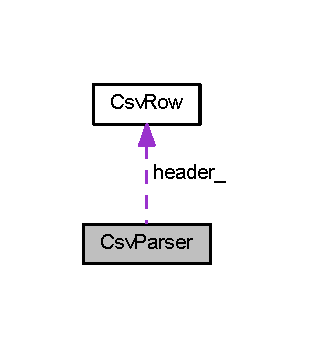
\includegraphics[width=149pt]{struct_csv_parser__coll__graph}
\end{center}
\end{figure}
\subsection*{Data Fields}
\begin{DoxyCompactItemize}
\item 
\mbox{\Hypertarget{struct_csv_parser_af8e15bff530b2aa132ee1ae6d9c55b4e}\label{struct_csv_parser_af8e15bff530b2aa132ee1ae6d9c55b4e}} 
char $\ast$ {\bfseries file\+Path\+\_\+}
\item 
\mbox{\Hypertarget{struct_csv_parser_a26fdea54e16baaffe0ed9119c0e9d4e5}\label{struct_csv_parser_a26fdea54e16baaffe0ed9119c0e9d4e5}} 
char {\bfseries delimiter\+\_\+}
\item 
\mbox{\Hypertarget{struct_csv_parser_ab6121214d4ead9cbe96afd9a920f92c7}\label{struct_csv_parser_ab6121214d4ead9cbe96afd9a920f92c7}} 
int {\bfseries first\+Line\+Is\+Header\+\_\+}
\item 
\mbox{\Hypertarget{struct_csv_parser_a3d80c0e7b25466b0ce505e419d93c6bf}\label{struct_csv_parser_a3d80c0e7b25466b0ce505e419d93c6bf}} 
char $\ast$ {\bfseries err\+Msg\+\_\+}
\item 
\mbox{\Hypertarget{struct_csv_parser_a2fee9340b04585bf3c349c28dbbe04bb}\label{struct_csv_parser_a2fee9340b04585bf3c349c28dbbe04bb}} 
\hyperlink{struct_csv_row}{Csv\+Row} $\ast$ {\bfseries header\+\_\+}
\item 
\mbox{\Hypertarget{struct_csv_parser_a25e2f4799c8893469b28666282accc20}\label{struct_csv_parser_a25e2f4799c8893469b28666282accc20}} 
F\+I\+LE $\ast$ {\bfseries file\+Handler\+\_\+}
\item 
\mbox{\Hypertarget{struct_csv_parser_a0e7996f7fb2622fb38f2f292cb04ce8b}\label{struct_csv_parser_a0e7996f7fb2622fb38f2f292cb04ce8b}} 
int {\bfseries from\+String\+\_\+}
\item 
\mbox{\Hypertarget{struct_csv_parser_a45eb545400de372945c3b5465ba0a5f0}\label{struct_csv_parser_a45eb545400de372945c3b5465ba0a5f0}} 
char $\ast$ {\bfseries csv\+String\+\_\+}
\item 
\mbox{\Hypertarget{struct_csv_parser_a0b405b96a2b250825fc5a185ce037603}\label{struct_csv_parser_a0b405b96a2b250825fc5a185ce037603}} 
int {\bfseries csv\+String\+Iter\+\_\+}
\end{DoxyCompactItemize}


\subsection{Detailed Description}


Definition at line 26 of file csvparser.\+h.



The documentation for this struct was generated from the following file\+:\begin{DoxyCompactItemize}
\item 
G\+:/\+Gen\+\_\+6-\/\+R\+\_\+\+I\+K\+\_\+\+Codes/\+New folder/\+Examples/example1/csvparser.\+h\end{DoxyCompactItemize}

\hypertarget{struct_csv_row}{}\section{Csv\+Row Struct Reference}
\label{struct_csv_row}\index{Csv\+Row@{Csv\+Row}}
\subsection*{Data Fields}
\begin{DoxyCompactItemize}
\item 
\mbox{\Hypertarget{struct_csv_row_a7e963d2c7107189e89528fcef40fd54e}\label{struct_csv_row_a7e963d2c7107189e89528fcef40fd54e}} 
char $\ast$$\ast$ {\bfseries fields\+\_\+}
\item 
\mbox{\Hypertarget{struct_csv_row_a10a8fa7afefe9385109a97d4354d6da6}\label{struct_csv_row_a10a8fa7afefe9385109a97d4354d6da6}} 
int {\bfseries num\+Of\+Fields\+\_\+}
\end{DoxyCompactItemize}


\subsection{Detailed Description}


Definition at line 21 of file csvparser.\+h.



The documentation for this struct was generated from the following file\+:\begin{DoxyCompactItemize}
\item 
G\+:/\+Gen\+\_\+6-\/\+R\+\_\+\+I\+K\+\_\+\+Codes/\+New folder/\+Examples/example1/csvparser.\+h\end{DoxyCompactItemize}

\hypertarget{struct_residue}{}\section{Residue Struct Reference}
\label{struct_residue}\index{Residue@{Residue}}


{\ttfamily \#include $<$cx.\+h$>$}

\subsection*{Data Fields}
\begin{DoxyCompactItemize}
\item 
\mbox{\Hypertarget{struct_residue_ac9c29659e079dc6581f430fbc14e5868}\label{struct_residue_ac9c29659e079dc6581f430fbc14e5868}} 
double \+\_\+\+Complex {\bfseries residue1}
\item 
\mbox{\Hypertarget{struct_residue_a8fd51b76ab87fcccdd236a49f6702c4b}\label{struct_residue_a8fd51b76ab87fcccdd236a49f6702c4b}} 
double \+\_\+\+Complex {\bfseries residue2}
\item 
\mbox{\Hypertarget{struct_residue_aedacac63d44a2c9da63dde018b805abb}\label{struct_residue_aedacac63d44a2c9da63dde018b805abb}} 
double \+\_\+\+Complex {\bfseries residue3}
\item 
\mbox{\Hypertarget{struct_residue_a76d6fcce21bba06dea1562aa50eaece0}\label{struct_residue_a76d6fcce21bba06dea1562aa50eaece0}} 
double \+\_\+\+Complex {\bfseries residue4}
\item 
\mbox{\Hypertarget{struct_residue_aaa02698cd0a5f95c444810d77efe8b02}\label{struct_residue_aaa02698cd0a5f95c444810d77efe8b02}} 
double \+\_\+\+Complex {\bfseries residue5}
\item 
\mbox{\Hypertarget{struct_residue_a41a6f986ca1f77d6154377d9dd9f9c7f}\label{struct_residue_a41a6f986ca1f77d6154377d9dd9f9c7f}} 
double \+\_\+\+Complex {\bfseries residue6}
\end{DoxyCompactItemize}


\subsection{Detailed Description}
\hyperlink{struct_residue}{Residue}\+: Structure type variable, to store residue1 to residue6, calculated from the six corresponding equations mentioned in the paper by Manocha and Canny.

Variables used\+: \tabulinesep=1mm
\begin{longtabu} spread 0pt [c]{*{2}{|X[-1]}|}
\hline
\rowcolor{\tableheadbgcolor}\textbf{ Variable }&\textbf{ Description  }\\\cline{1-2}
\endfirsthead
\hline
\endfoot
\hline
\rowcolor{\tableheadbgcolor}\textbf{ Variable }&\textbf{ Description  }\\\cline{1-2}
\endhead
residue1 &Variable to store residue1. \\\cline{1-2}
residue2 &Variable to store residue2. \\\cline{1-2}
residue3 &Variable to store residue3. \\\cline{1-2}
residue4 &Variable to store residue4. \\\cline{1-2}
residue5 &Variable to store residue5. \\\cline{1-2}
residue6 &Variable to store residue6. \\\cline{1-2}
\end{longtabu}


Definition at line 76 of file cx.\+h.



The documentation for this struct was generated from the following file\+:\begin{DoxyCompactItemize}
\item 
G\+:/\+Gen\+\_\+6-\/\+R\+\_\+\+I\+K\+\_\+\+Codes/\+New folder/\+Examples/example1/cx.\+h\end{DoxyCompactItemize}

\hypertarget{struct_solution}{}\section{Solution Struct Reference}
\label{struct_solution}\index{Solution@{Solution}}


{\ttfamily \#include $<$cx.\+h$>$}

\subsection*{Data Fields}
\begin{DoxyCompactItemize}
\item 
\mbox{\Hypertarget{struct_solution_a1ce2dc2e3874867ac9c9c10d4152e285}\label{struct_solution_a1ce2dc2e3874867ac9c9c10d4152e285}} 
double \+\_\+\+Complex {\bfseries thetar} \mbox{[}20\mbox{]}\mbox{[}10\mbox{]}
\item 
\mbox{\Hypertarget{struct_solution_aab13a66a6f49c2222e26cebc1db1468d}\label{struct_solution_aab13a66a6f49c2222e26cebc1db1468d}} 
double \+\_\+\+Complex {\bfseries thetad} \mbox{[}20\mbox{]}\mbox{[}10\mbox{]}
\item 
\mbox{\Hypertarget{struct_solution_a93572d193d49e1c5672276bb34b9a3cf}\label{struct_solution_a93572d193d49e1c5672276bb34b9a3cf}} 
double \+\_\+\+Complex {\bfseries residue} \mbox{[}20\mbox{]}\mbox{[}10\mbox{]}
\end{DoxyCompactItemize}


\subsection{Detailed Description}
\hyperlink{struct_solution}{Solution}\+: Structure type variable, to store the six joint angles in radians, the six joint angles in degrees, and the six residues for all the branches of the inverse kinematics solution.

Variables used\+: \tabulinesep=1mm
\begin{longtabu} spread 0pt [c]{*{2}{|X[-1]}|}
\hline
\rowcolor{\tableheadbgcolor}\textbf{ Variable }&\textbf{ Description  }\\\cline{1-2}
\endfirsthead
\hline
\endfoot
\hline
\rowcolor{\tableheadbgcolor}\textbf{ Variable }&\textbf{ Description  }\\\cline{1-2}
\endhead
thetar &A 2-\/D array to store the six joint angles (in radians) for all the branches of the inverse kinematics solution. \\\cline{1-2}
thetad &A 2-\/D array to store the six joint angles (in degrees) for all the branches of the inverse kinematics solution. \\\cline{1-2}
residue &A 2-\/D array to store the six residues for for all the branches of the inverse kinematics solution. \\\cline{1-2}
\end{longtabu}


Definition at line 32 of file cx.\+h.



The documentation for this struct was generated from the following file\+:\begin{DoxyCompactItemize}
\item 
G\+:/\+Gen\+\_\+6-\/\+R\+\_\+\+I\+K\+\_\+\+Codes/\+New folder/\+Examples/example1/cx.\+h\end{DoxyCompactItemize}

\hypertarget{struct_theta}{}\section{Theta Struct Reference}
\label{struct_theta}\index{Theta@{Theta}}


{\ttfamily \#include $<$cx.\+h$>$}

\subsection*{Data Fields}
\begin{DoxyCompactItemize}
\item 
\mbox{\Hypertarget{struct_theta_a52d5fcaad2bc567dddde4c74c1a67919}\label{struct_theta_a52d5fcaad2bc567dddde4c74c1a67919}} 
double \+\_\+\+Complex {\bfseries sintheta}
\item 
\mbox{\Hypertarget{struct_theta_a9b9955bdf805e7dc574b6edf2277638f}\label{struct_theta_a9b9955bdf805e7dc574b6edf2277638f}} 
double \+\_\+\+Complex {\bfseries costheta}
\end{DoxyCompactItemize}


\subsection{Detailed Description}
\hyperlink{struct_theta}{Theta}\+: Structure type variable, to store the sin(theta) and cos(theta) outputs from the functions, \textquotesingle{}theta1\textquotesingle{}, \textquotesingle{}theta2\textquotesingle{} and \textquotesingle{}theta6\textquotesingle{}.

Variables used\+: \tabulinesep=1mm
\begin{longtabu} spread 0pt [c]{*{2}{|X[-1]}|}
\hline
\rowcolor{\tableheadbgcolor}\textbf{ Variable }&\textbf{ Description  }\\\cline{1-2}
\endfirsthead
\hline
\endfoot
\hline
\rowcolor{\tableheadbgcolor}\textbf{ Variable }&\textbf{ Description  }\\\cline{1-2}
\endhead
sintheta &Variable to store sin(theta). \\\cline{1-2}
costheta &Variable to store cos(theta). \\\cline{1-2}
\end{longtabu}


Definition at line 53 of file cx.\+h.



The documentation for this struct was generated from the following file\+:\begin{DoxyCompactItemize}
\item 
G\+:/\+Gen\+\_\+6-\/\+R\+\_\+\+I\+K\+\_\+\+Codes/\+New folder/\+Examples/example1/cx.\+h\end{DoxyCompactItemize}

\chapter{File Documentation}
\hypertarget{example1_8c}{}\section{G\+:/\+Gen\+\_\+6-\/\+R\+\_\+\+I\+K\+\_\+\+Codes/\+New folder/\+Examples/example1/example1.c File Reference}
\label{example1_8c}\index{G\+:/\+Gen\+\_\+6-\/\+R\+\_\+\+I\+K\+\_\+\+Codes/\+New folder/\+Examples/example1/example1.\+c@{G\+:/\+Gen\+\_\+6-\/\+R\+\_\+\+I\+K\+\_\+\+Codes/\+New folder/\+Examples/example1/example1.\+c}}


This file demonstrates the use of the Inverse kinematics function Inverse\+Kinematics\+General6R, through an example on a general 6-\/R serial manipulator, taken from the 1990 paper by \textquotesingle{}Raghavan and Roth\textquotesingle{}.  


{\ttfamily \#include \char`\"{}cx.\+h\char`\"{}}\newline
{\ttfamily \#include \char`\"{}csvparser.\+h\char`\"{}}\newline
{\ttfamily \#include $<$stdio.\+h$>$}\newline
{\ttfamily \#include $<$string.\+h$>$}\newline
{\ttfamily \#include $<$stdlib.\+h$>$}\newline
{\ttfamily \#include $<$math.\+h$>$}\newline
{\ttfamily \#include $<$complex.\+h$>$}\newline
{\ttfamily \#include $<$gsl/gsl\+\_\+math.\+h$>$}\newline
{\ttfamily \#include $<$gsl/gsl\+\_\+eigen.\+h$>$}\newline
{\ttfamily \#include $<$gsl/gsl\+\_\+vector.\+h$>$}\newline
{\ttfamily \#include $<$gsl/gsl\+\_\+complex.\+h$>$}\newline
{\ttfamily \#include $<$gsl/gsl\+\_\+complex\+\_\+math.\+h$>$}\newline
{\ttfamily \#include $<$gsl/gsl\+\_\+statistics.\+h$>$}\newline
{\ttfamily \#include $<$time.\+h$>$}\newline
Include dependency graph for example1.\+c\+:\nopagebreak
\begin{figure}[H]
\begin{center}
\leavevmode
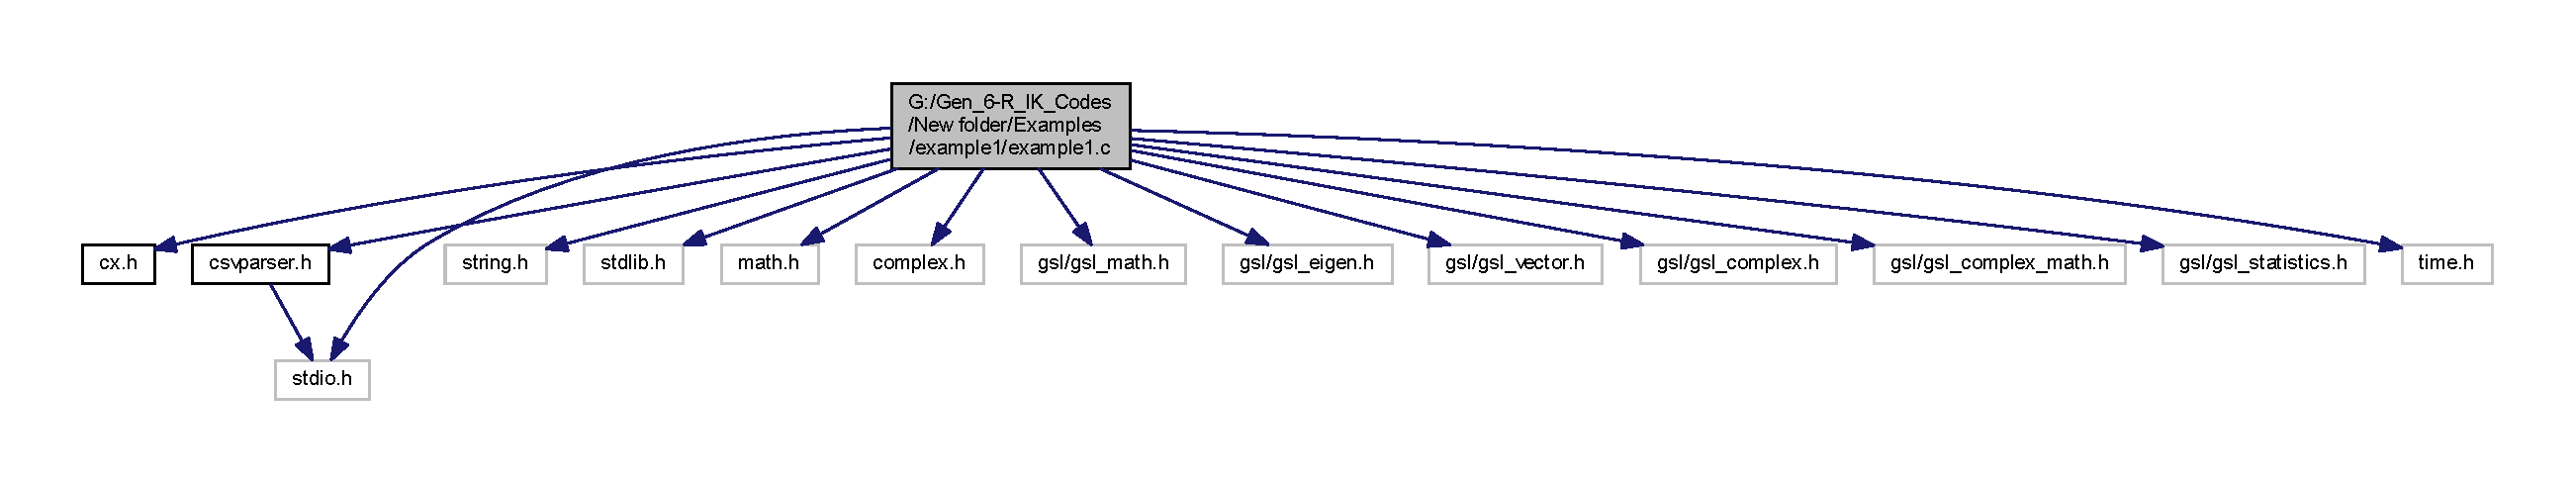
\includegraphics[width=350pt]{example1_8c__incl}
\end{center}
\end{figure}
\subsection*{Functions}
\begin{DoxyCompactItemize}
\item 
void \hyperlink{example1_8c_ab70a879cab358334de3af0cbcda7d189}{create\+\_\+csv} (char $\ast$filename, double \+\_\+\+Complex solution\mbox{[}$\,$\mbox{]}\mbox{[}10\mbox{]}, int n, int m)
\item 
int \hyperlink{example1_8c_ae66f6b31b5ad750f1fe042a706a4e3d4}{main} ()
\end{DoxyCompactItemize}


\subsection{Detailed Description}
This file demonstrates the use of the Inverse kinematics function Inverse\+Kinematics\+General6R, through an example on a general 6-\/R serial manipulator, taken from the 1990 paper by \textquotesingle{}Raghavan and Roth\textquotesingle{}. 

\begin{DoxyDate}{Date}
September 30, 2017 
\end{DoxyDate}


\subsection{Function Documentation}
\mbox{\Hypertarget{example1_8c_ab70a879cab358334de3af0cbcda7d189}\label{example1_8c_ab70a879cab358334de3af0cbcda7d189}} 
\index{example1.\+c@{example1.\+c}!create\+\_\+csv@{create\+\_\+csv}}
\index{create\+\_\+csv@{create\+\_\+csv}!example1.\+c@{example1.\+c}}
\subsubsection{\texorpdfstring{create\+\_\+csv()}{create\_csv()}}
{\footnotesize\ttfamily void create\+\_\+csv (\begin{DoxyParamCaption}\item[{char $\ast$}]{filename,  }\item[{double \+\_\+\+Complex}]{solution\mbox{[}$\,$\mbox{]}\mbox{[}10\mbox{]},  }\item[{int}]{n,  }\item[{int}]{m }\end{DoxyParamCaption})}

create\+\_\+csv\+: Function to create a C\+SV file.


\begin{DoxyParams}{Parameters}
{\em filename} & Name of the C\+SV file to be generated. \\
\hline
{\em solution} & A 2-\/D array containing the information to be stored in the C\+SV file. \\
\hline
{\em m} & No. of rows of the above defined 2-\/D array \textquotesingle{}solution\textquotesingle{}. \\
\hline
{\em n} & No. of columns of the above defined 2-\/D array \textquotesingle{}solution\textquotesingle{}.\\
\hline
\end{DoxyParams}
Variables used\+: \tabulinesep=1mm
\begin{longtabu} spread 0pt [c]{*{2}{|X[-1]}|}
\hline
\rowcolor{\tableheadbgcolor}\textbf{ Variable }&\textbf{ Description  }\\\cline{1-2}
\endfirsthead
\hline
\endfoot
\hline
\rowcolor{\tableheadbgcolor}\textbf{ Variable }&\textbf{ Description  }\\\cline{1-2}
\endhead
fp &A pointer of type F\+I\+LE to hold the C\+SV file named \textquotesingle{}filename\textquotesingle{}, which is an user input. \\\cline{1-2}
\end{longtabu}


\begin{DoxyReturn}{Returns}
\+: The C\+SV file thus created. 
\end{DoxyReturn}


Definition at line 48 of file example1.\+c.

Here is the caller graph for this function\+:\nopagebreak
\begin{figure}[H]
\begin{center}
\leavevmode
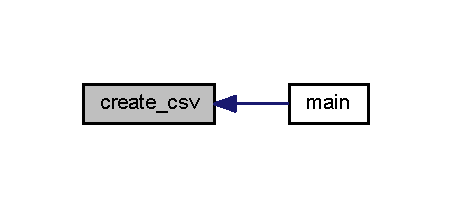
\includegraphics[width=217pt]{example1_8c_ab70a879cab358334de3af0cbcda7d189_icgraph}
\end{center}
\end{figure}
\mbox{\Hypertarget{example1_8c_ae66f6b31b5ad750f1fe042a706a4e3d4}\label{example1_8c_ae66f6b31b5ad750f1fe042a706a4e3d4}} 
\index{example1.\+c@{example1.\+c}!main@{main}}
\index{main@{main}!example1.\+c@{example1.\+c}}
\subsubsection{\texorpdfstring{main()}{main()}}
{\footnotesize\ttfamily int main (\begin{DoxyParamCaption}{ }\end{DoxyParamCaption})}

main program to demonstrate the usage of the function \textquotesingle{}Inverse\+Kinematics\+General6R\textquotesingle{}.

For computing the inverse kinematics of any other general 6-\/R robot, the C\+SV file containing the D-\/H parameters needs to be placed at the position of \textquotesingle{}dhmat\+\_\+\+Raghavan\+\_\+\+Roth.\+csv\textquotesingle{} in the program below, and for any other End-\/effector pose of the robot, the C\+SV file containing the End-\/effector pose needs to be placed at the position of \textquotesingle{}eemat\+\_\+\+Raghavan\+\_\+\+Roth.\+csv\textquotesingle{}. The way to input D-\/H parameters and the End-\/\+Effector pose into the corresponding C\+SV files has been explained in the document \textquotesingle{}I\+K\+\_\+6\+R\+\_\+\+Program\+\_\+\+Documentation.\+pdf\textquotesingle{}.

Variables used\+: \tabulinesep=1mm
\begin{longtabu} spread 0pt [c]{*{2}{|X[-1]}|}
\hline
\rowcolor{\tableheadbgcolor}\textbf{ Variable }&\textbf{ Description  }\\\cline{1-2}
\endfirsthead
\hline
\endfoot
\hline
\rowcolor{\tableheadbgcolor}\textbf{ Variable }&\textbf{ Description  }\\\cline{1-2}
\endhead
soln &Structure type variable, to store the output of the function \textquotesingle{}Inverse\+Kinematics\+General6R\textquotesingle{}. Its definition is there in the header file, \textquotesingle{}cx.\+h\textquotesingle{}. \\\cline{1-2}
start, end, cpu\+\_\+time\+\_\+used &To calculate the average computation time of the inverse kinematics solution through the use of the function \textquotesingle{}Inverse\+Kinematics\+General6R\textquotesingle{} \\\cline{1-2}
NN &No. of cycles over which the function \textquotesingle{}Inverse\+Kinematics\+General6R\textquotesingle{} has been evaluated to get an estimate of its average computation time. \\\cline{1-2}
\end{longtabu}


Definition at line 107 of file example1.\+c.

Here is the call graph for this function\+:\nopagebreak
\begin{figure}[H]
\begin{center}
\leavevmode
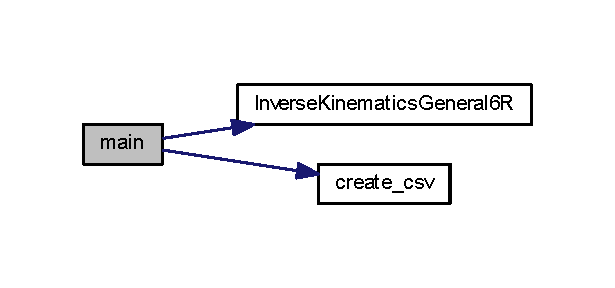
\includegraphics[width=295pt]{example1_8c_ae66f6b31b5ad750f1fe042a706a4e3d4_cgraph}
\end{center}
\end{figure}

\hypertarget{example2_8c}{}\section{G\+:/\+Gen\+\_\+6-\/\+R\+\_\+\+I\+K\+\_\+\+Codes/\+New folder/\+Examples/example2/example2.c File Reference}
\label{example2_8c}\index{G\+:/\+Gen\+\_\+6-\/\+R\+\_\+\+I\+K\+\_\+\+Codes/\+New folder/\+Examples/example2/example2.\+c@{G\+:/\+Gen\+\_\+6-\/\+R\+\_\+\+I\+K\+\_\+\+Codes/\+New folder/\+Examples/example2/example2.\+c}}


This file demonstrates the use of the Inverse kinematics function \textquotesingle{}Inverse\+Kinematics\+General6R\textquotesingle{}, through an example on a general 6-\/R serial manipulator, taken from the 2007 paper by \textquotesingle{}Liu and Zhu\textquotesingle{}, on this topic.  


{\ttfamily \#include \char`\"{}cx.\+h\char`\"{}}\newline
{\ttfamily \#include \char`\"{}csvparser.\+h\char`\"{}}\newline
{\ttfamily \#include $<$stdio.\+h$>$}\newline
{\ttfamily \#include $<$string.\+h$>$}\newline
{\ttfamily \#include $<$stdlib.\+h$>$}\newline
{\ttfamily \#include $<$math.\+h$>$}\newline
{\ttfamily \#include $<$complex.\+h$>$}\newline
{\ttfamily \#include $<$gsl/gsl\+\_\+math.\+h$>$}\newline
{\ttfamily \#include $<$gsl/gsl\+\_\+eigen.\+h$>$}\newline
{\ttfamily \#include $<$gsl/gsl\+\_\+vector.\+h$>$}\newline
{\ttfamily \#include $<$gsl/gsl\+\_\+complex.\+h$>$}\newline
{\ttfamily \#include $<$gsl/gsl\+\_\+complex\+\_\+math.\+h$>$}\newline
{\ttfamily \#include $<$gsl/gsl\+\_\+statistics.\+h$>$}\newline
{\ttfamily \#include $<$time.\+h$>$}\newline
Include dependency graph for example2.\+c\+:\nopagebreak
\begin{figure}[H]
\begin{center}
\leavevmode
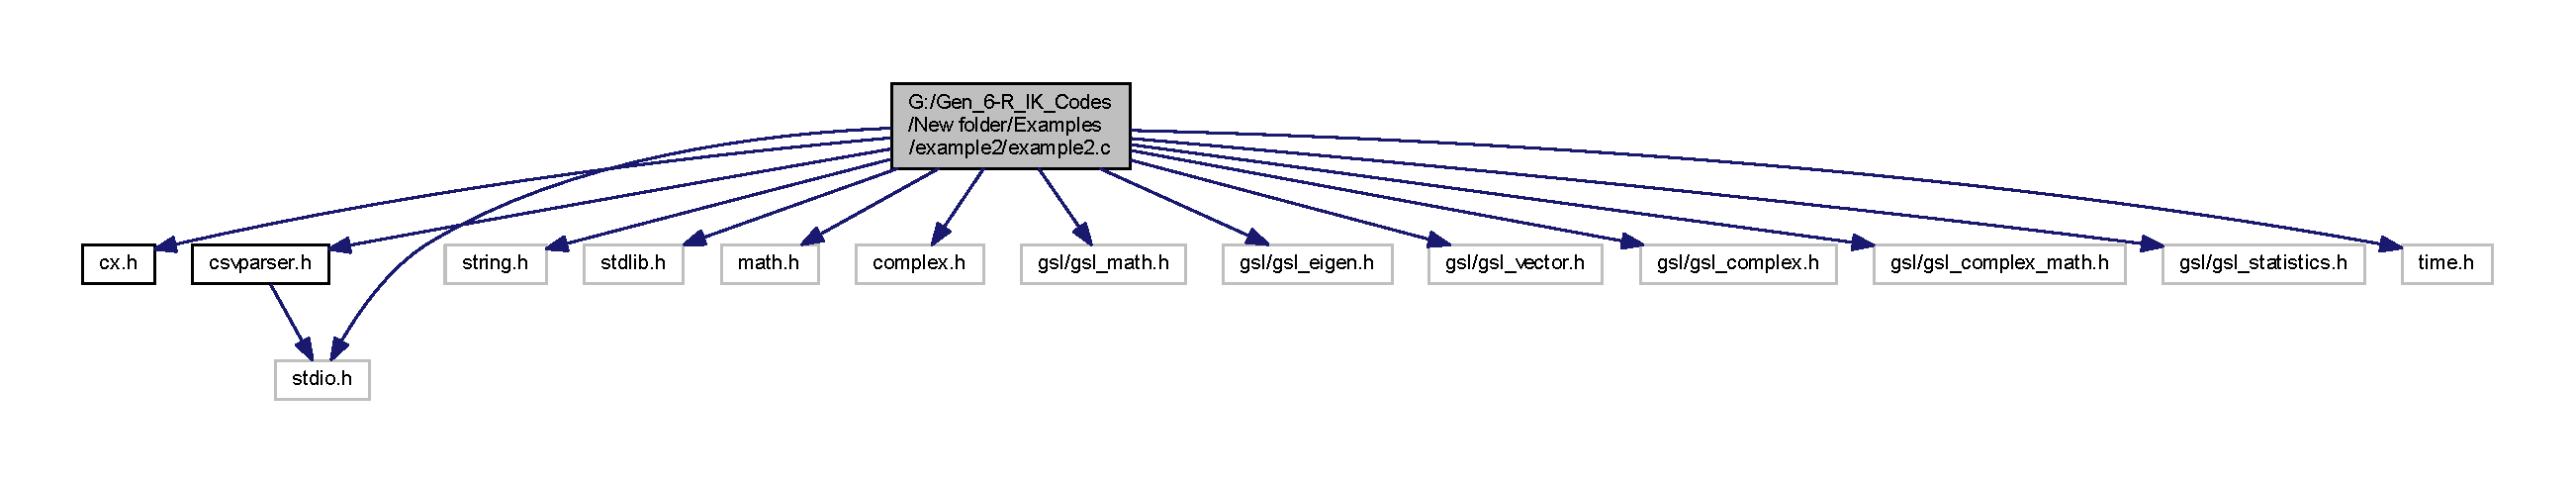
\includegraphics[width=350pt]{example2_8c__incl}
\end{center}
\end{figure}
\subsection*{Functions}
\begin{DoxyCompactItemize}
\item 
void \hyperlink{example2_8c_ab70a879cab358334de3af0cbcda7d189}{create\+\_\+csv} (char $\ast$filename, double \+\_\+\+Complex solution\mbox{[}$\,$\mbox{]}\mbox{[}10\mbox{]}, int n, int m)
\item 
int \hyperlink{example2_8c_ae66f6b31b5ad750f1fe042a706a4e3d4}{main} ()
\end{DoxyCompactItemize}


\subsection{Detailed Description}
This file demonstrates the use of the Inverse kinematics function \textquotesingle{}Inverse\+Kinematics\+General6R\textquotesingle{}, through an example on a general 6-\/R serial manipulator, taken from the 2007 paper by \textquotesingle{}Liu and Zhu\textquotesingle{}, on this topic. 

\begin{DoxyDate}{Date}
September 30, 2017 
\end{DoxyDate}


\subsection{Function Documentation}
\mbox{\Hypertarget{example2_8c_ab70a879cab358334de3af0cbcda7d189}\label{example2_8c_ab70a879cab358334de3af0cbcda7d189}} 
\index{example2.\+c@{example2.\+c}!create\+\_\+csv@{create\+\_\+csv}}
\index{create\+\_\+csv@{create\+\_\+csv}!example2.\+c@{example2.\+c}}
\subsubsection{\texorpdfstring{create\+\_\+csv()}{create\_csv()}}
{\footnotesize\ttfamily void create\+\_\+csv (\begin{DoxyParamCaption}\item[{char $\ast$}]{filename,  }\item[{double \+\_\+\+Complex}]{solution\mbox{[}$\,$\mbox{]}\mbox{[}10\mbox{]},  }\item[{int}]{n,  }\item[{int}]{m }\end{DoxyParamCaption})}

create\+\_\+csv\+: Function to create a C\+SV file.


\begin{DoxyParams}{Parameters}
{\em filename} & Name of the C\+SV file to be generated. \\
\hline
{\em solution} & A 2-\/D array containing the information to be stored in the C\+SV file. \\
\hline
{\em m} & No. of rows of the above defined 2-\/D array \textquotesingle{}solution\textquotesingle{}. \\
\hline
{\em n} & No. of columns of the above defined 2-\/D array \textquotesingle{}solution\textquotesingle{}.\\
\hline
\end{DoxyParams}
Variables used\+: \tabulinesep=1mm
\begin{longtabu} spread 0pt [c]{*{2}{|X[-1]}|}
\hline
\rowcolor{\tableheadbgcolor}\textbf{ Variable }&\textbf{ Description  }\\\cline{1-2}
\endfirsthead
\hline
\endfoot
\hline
\rowcolor{\tableheadbgcolor}\textbf{ Variable }&\textbf{ Description  }\\\cline{1-2}
\endhead
fp &A pointer of type F\+I\+LE to hold the C\+SV file named \textquotesingle{}filename\textquotesingle{}, which is an user input. \\\cline{1-2}
\end{longtabu}


\begin{DoxyReturn}{Returns}
\+: The C\+SV file thus created. 
\end{DoxyReturn}


Definition at line 48 of file example2.\+c.

Here is the caller graph for this function\+:\nopagebreak
\begin{figure}[H]
\begin{center}
\leavevmode
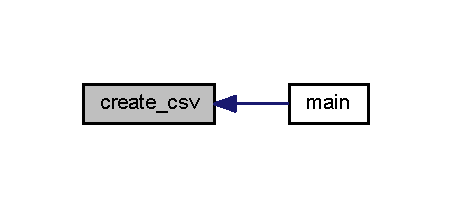
\includegraphics[width=217pt]{example2_8c_ab70a879cab358334de3af0cbcda7d189_icgraph}
\end{center}
\end{figure}
\mbox{\Hypertarget{example2_8c_ae66f6b31b5ad750f1fe042a706a4e3d4}\label{example2_8c_ae66f6b31b5ad750f1fe042a706a4e3d4}} 
\index{example2.\+c@{example2.\+c}!main@{main}}
\index{main@{main}!example2.\+c@{example2.\+c}}
\subsubsection{\texorpdfstring{main()}{main()}}
{\footnotesize\ttfamily int main (\begin{DoxyParamCaption}{ }\end{DoxyParamCaption})}

main program to demonstrate the usage of the function Inverse\+Kinematics\+General6R.

For computing the inverse kinematics of any other general 6-\/R robot, the C\+SV file containing the D-\/H parameters needs to be placed at the position of \textquotesingle{}dhmat\+\_\+\+Raghavan\+\_\+\+Roth.\+csv\textquotesingle{} in the program below, and for any other End-\/effector pose of the robot, the C\+SV file containing the End-\/effector pose needs to be placed at the position of \textquotesingle{}eemat\+\_\+\+Raghavan\+\_\+\+Roth.\+csv\textquotesingle{}. The way to input D-\/H parameters and the End-\/\+Effector pose into the corresponding C\+SV files has been explained in the document \textquotesingle{}I\+K\+\_\+6\+R\+\_\+\+Program\+\_\+\+Documentation.\+pdf\textquotesingle{}.

Variables used\+: \tabulinesep=1mm
\begin{longtabu} spread 0pt [c]{*{2}{|X[-1]}|}
\hline
\rowcolor{\tableheadbgcolor}\textbf{ Variable }&\textbf{ Description  }\\\cline{1-2}
\endfirsthead
\hline
\endfoot
\hline
\rowcolor{\tableheadbgcolor}\textbf{ Variable }&\textbf{ Description  }\\\cline{1-2}
\endhead
soln &Structure type variable, to store the output of the function Inverse\+Kinematics\+General6R. Its definition is there in the header file, \textquotesingle{}cx.\+h\textquotesingle{}. \\\cline{1-2}
start, end, cpu\+\_\+time\+\_\+used &To calculate the average computation time of the inverse kinematics solution through the use of the function Inverse\+Kinematics\+General6R \\\cline{1-2}
NN &No. of cycles over which the function Inverse\+Kinematics\+General6R has been evaluated to get an estimate of its average computation time. \\\cline{1-2}
\end{longtabu}


Definition at line 107 of file example2.\+c.

Here is the call graph for this function\+:\nopagebreak
\begin{figure}[H]
\begin{center}
\leavevmode
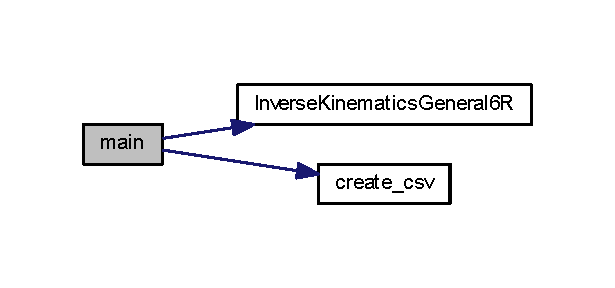
\includegraphics[width=295pt]{example2_8c_ae66f6b31b5ad750f1fe042a706a4e3d4_cgraph}
\end{center}
\end{figure}

\hypertarget{example3_8c}{}\section{G\+:/\+Gen\+\_\+6-\/\+R\+\_\+\+I\+K\+\_\+\+Codes/\+New folder/\+Examples/example3\+\_\+\+Jaco/example3.c File Reference}
\label{example3_8c}\index{G\+:/\+Gen\+\_\+6-\/\+R\+\_\+\+I\+K\+\_\+\+Codes/\+New folder/\+Examples/example3\+\_\+\+Jaco/example3.\+c@{G\+:/\+Gen\+\_\+6-\/\+R\+\_\+\+I\+K\+\_\+\+Codes/\+New folder/\+Examples/example3\+\_\+\+Jaco/example3.\+c}}


This file demonstrates the use of the Inverse kinematics function \textquotesingle{}Inverse\+Kinematics\+General6R\textquotesingle{}, through an example on the general 6-\/R serial manipulator, Jaco. For this manipulator the D-\/H parameter a1 = 0 m. For this algorithm to work, \textquotesingle{}a1\textquotesingle{} is taken as 0.\+001 m, and it is found that the residues still are of the order of 10$^\wedge$-\/6.  


{\ttfamily \#include \char`\"{}cx.\+h\char`\"{}}\newline
{\ttfamily \#include \char`\"{}csvparser.\+h\char`\"{}}\newline
{\ttfamily \#include $<$stdio.\+h$>$}\newline
{\ttfamily \#include $<$string.\+h$>$}\newline
{\ttfamily \#include $<$stdlib.\+h$>$}\newline
{\ttfamily \#include $<$math.\+h$>$}\newline
{\ttfamily \#include $<$complex.\+h$>$}\newline
{\ttfamily \#include $<$gsl/gsl\+\_\+math.\+h$>$}\newline
{\ttfamily \#include $<$gsl/gsl\+\_\+eigen.\+h$>$}\newline
{\ttfamily \#include $<$gsl/gsl\+\_\+vector.\+h$>$}\newline
{\ttfamily \#include $<$gsl/gsl\+\_\+complex.\+h$>$}\newline
{\ttfamily \#include $<$gsl/gsl\+\_\+complex\+\_\+math.\+h$>$}\newline
{\ttfamily \#include $<$gsl/gsl\+\_\+statistics.\+h$>$}\newline
{\ttfamily \#include $<$time.\+h$>$}\newline
Include dependency graph for example3.\+c\+:\nopagebreak
\begin{figure}[H]
\begin{center}
\leavevmode
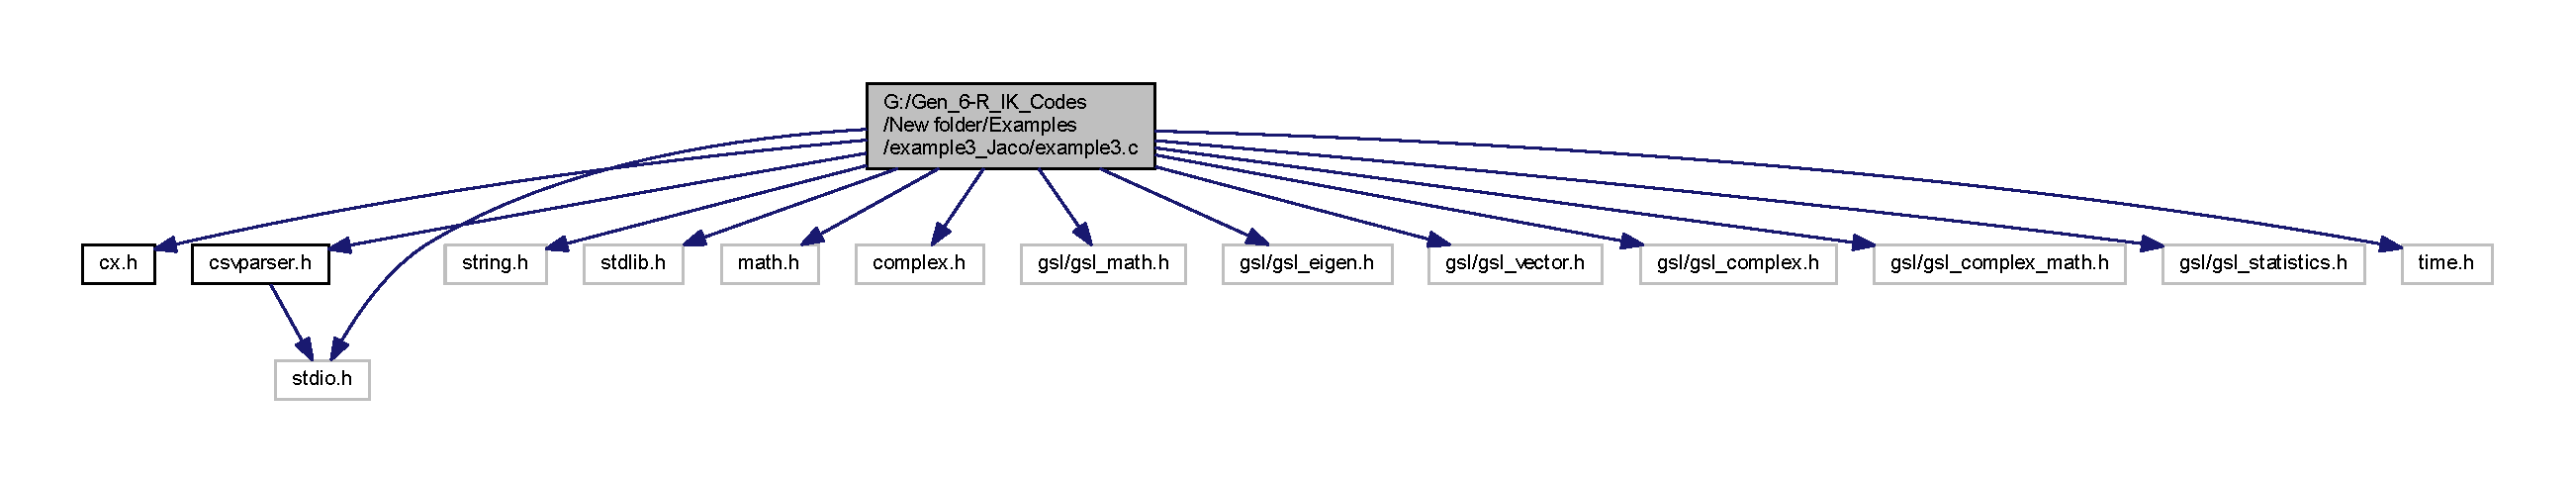
\includegraphics[width=350pt]{example3_8c__incl}
\end{center}
\end{figure}
\subsection*{Functions}
\begin{DoxyCompactItemize}
\item 
void \hyperlink{example3_8c_ab70a879cab358334de3af0cbcda7d189}{create\+\_\+csv} (char $\ast$filename, double \+\_\+\+Complex solution\mbox{[}$\,$\mbox{]}\mbox{[}10\mbox{]}, int n, int m)
\item 
int \hyperlink{example3_8c_ae66f6b31b5ad750f1fe042a706a4e3d4}{main} ()
\end{DoxyCompactItemize}


\subsection{Detailed Description}
This file demonstrates the use of the Inverse kinematics function \textquotesingle{}Inverse\+Kinematics\+General6R\textquotesingle{}, through an example on the general 6-\/R serial manipulator, Jaco. For this manipulator the D-\/H parameter a1 = 0 m. For this algorithm to work, \textquotesingle{}a1\textquotesingle{} is taken as 0.\+001 m, and it is found that the residues still are of the order of 10$^\wedge$-\/6. 

\begin{DoxyDate}{Date}
September 30, 2017 
\end{DoxyDate}


\subsection{Function Documentation}
\mbox{\Hypertarget{example3_8c_ab70a879cab358334de3af0cbcda7d189}\label{example3_8c_ab70a879cab358334de3af0cbcda7d189}} 
\index{example3.\+c@{example3.\+c}!create\+\_\+csv@{create\+\_\+csv}}
\index{create\+\_\+csv@{create\+\_\+csv}!example3.\+c@{example3.\+c}}
\subsubsection{\texorpdfstring{create\+\_\+csv()}{create\_csv()}}
{\footnotesize\ttfamily void create\+\_\+csv (\begin{DoxyParamCaption}\item[{char $\ast$}]{filename,  }\item[{double \+\_\+\+Complex}]{solution\mbox{[}$\,$\mbox{]}\mbox{[}10\mbox{]},  }\item[{int}]{n,  }\item[{int}]{m }\end{DoxyParamCaption})}

create\+\_\+csv\+: Function to create a C\+SV file.


\begin{DoxyParams}{Parameters}
{\em filename} & Name of the C\+SV file to be generated. \\
\hline
{\em solution} & A 2-\/D array containing the information to be stored in the C\+SV file. \\
\hline
{\em m} & No. of rows of the above defined 2-\/D array \textquotesingle{}solution\textquotesingle{}. \\
\hline
{\em n} & No. of columns of the above defined 2-\/D array \textquotesingle{}solution\textquotesingle{}.\\
\hline
\end{DoxyParams}
Variables used\+: \tabulinesep=1mm
\begin{longtabu} spread 0pt [c]{*{2}{|X[-1]}|}
\hline
\rowcolor{\tableheadbgcolor}\textbf{ Variable }&\textbf{ Description  }\\\cline{1-2}
\endfirsthead
\hline
\endfoot
\hline
\rowcolor{\tableheadbgcolor}\textbf{ Variable }&\textbf{ Description  }\\\cline{1-2}
\endhead
fp &A pointer of type F\+I\+LE to hold the C\+SV file named \textquotesingle{}filename\textquotesingle{}, which is an user input. \\\cline{1-2}
\end{longtabu}


\begin{DoxyReturn}{Returns}
\+: The C\+SV file thus created. 
\end{DoxyReturn}


Definition at line 49 of file example3.\+c.

Here is the caller graph for this function\+:\nopagebreak
\begin{figure}[H]
\begin{center}
\leavevmode
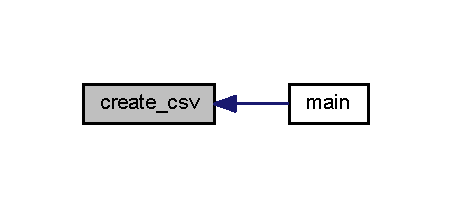
\includegraphics[width=217pt]{example3_8c_ab70a879cab358334de3af0cbcda7d189_icgraph}
\end{center}
\end{figure}
\mbox{\Hypertarget{example3_8c_ae66f6b31b5ad750f1fe042a706a4e3d4}\label{example3_8c_ae66f6b31b5ad750f1fe042a706a4e3d4}} 
\index{example3.\+c@{example3.\+c}!main@{main}}
\index{main@{main}!example3.\+c@{example3.\+c}}
\subsubsection{\texorpdfstring{main()}{main()}}
{\footnotesize\ttfamily int main (\begin{DoxyParamCaption}{ }\end{DoxyParamCaption})}

main program to demonstrate the usage of the function Inverse\+Kinematics\+General6R.

For computing the inverse kinematics of any other general 6-\/R robot, the C\+SV file containing the D-\/H parameters needs to be placed at the position of \textquotesingle{}dhmat\+\_\+\+Raghavan\+\_\+\+Roth.\+csv\textquotesingle{} in the program below, and for any other End-\/effector pose of the robot, the C\+SV file containing the End-\/effector pose needs to be placed at the position of \textquotesingle{}eemat\+\_\+\+Raghavan\+\_\+\+Roth.\+csv\textquotesingle{}. The way to input D-\/H parameters and the End-\/\+Effector pose into the corresponding C\+SV files has been explained in the document \textquotesingle{}I\+K\+\_\+6\+R\+\_\+\+Program\+\_\+\+Documentation.\+pdf\textquotesingle{}.

Variables used\+: \tabulinesep=1mm
\begin{longtabu} spread 0pt [c]{*{2}{|X[-1]}|}
\hline
\rowcolor{\tableheadbgcolor}\textbf{ Variable }&\textbf{ Description  }\\\cline{1-2}
\endfirsthead
\hline
\endfoot
\hline
\rowcolor{\tableheadbgcolor}\textbf{ Variable }&\textbf{ Description  }\\\cline{1-2}
\endhead
soln &Structure type variable, to store the output of the function Inverse\+Kinematics\+General6R. Its definition is there in the header file, \textquotesingle{}cx.\+h\textquotesingle{}. \\\cline{1-2}
start, end, cpu\+\_\+time\+\_\+used &To calculate the average computation time of the inverse kinematics solution through the use of the function Inverse\+Kinematics\+General6R \\\cline{1-2}
NN &No. of cycles over which the function Inverse\+Kinematics\+General6R has been evaluated to get an estimate of its average computation time. \\\cline{1-2}
\end{longtabu}


Definition at line 108 of file example3.\+c.

Here is the call graph for this function\+:\nopagebreak
\begin{figure}[H]
\begin{center}
\leavevmode
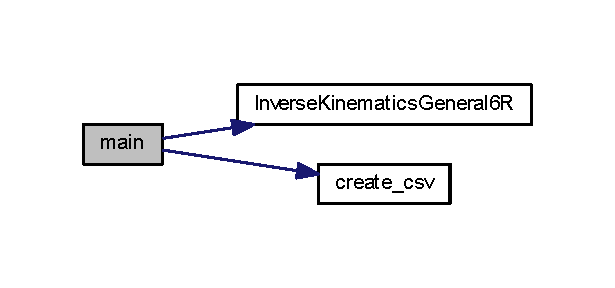
\includegraphics[width=295pt]{example3_8c_ae66f6b31b5ad750f1fe042a706a4e3d4_cgraph}
\end{center}
\end{figure}

\hypertarget{_inverse_kinematics_general6_r_8c}{}\section{G\+:/\+Gen\+\_\+6-\/\+R\+\_\+\+I\+K\+\_\+\+Codes/\+New folder/\+Examples/\+I\+K/\+Inverse\+Kinematics\+General6R.c File Reference}
\label{_inverse_kinematics_general6_r_8c}\index{G\+:/\+Gen\+\_\+6-\/\+R\+\_\+\+I\+K\+\_\+\+Codes/\+New folder/\+Examples/\+I\+K/\+Inverse\+Kinematics\+General6\+R.\+c@{G\+:/\+Gen\+\_\+6-\/\+R\+\_\+\+I\+K\+\_\+\+Codes/\+New folder/\+Examples/\+I\+K/\+Inverse\+Kinematics\+General6\+R.\+c}}


The program is used to find the Inverse kinematics solutions for a general 6-\/R serial manipulator.  


{\ttfamily \#include \char`\"{}cx.\+h\char`\"{}}\newline
{\ttfamily \#include $<$stdio.\+h$>$}\newline
{\ttfamily \#include $<$string.\+h$>$}\newline
{\ttfamily \#include $<$stdlib.\+h$>$}\newline
{\ttfamily \#include $<$math.\+h$>$}\newline
{\ttfamily \#include $<$complex.\+h$>$}\newline
{\ttfamily \#include $<$gsl/gsl\+\_\+math.\+h$>$}\newline
{\ttfamily \#include $<$gsl/gsl\+\_\+eigen.\+h$>$}\newline
{\ttfamily \#include $<$gsl/gsl\+\_\+vector.\+h$>$}\newline
{\ttfamily \#include $<$gsl/gsl\+\_\+complex.\+h$>$}\newline
{\ttfamily \#include $<$gsl/gsl\+\_\+complex\+\_\+math.\+h$>$}\newline
{\ttfamily \#include $<$gsl/gsl\+\_\+statistics.\+h$>$}\newline
Include dependency graph for Inverse\+Kinematics\+General6\+R.\+c\+:\nopagebreak
\begin{figure}[H]
\begin{center}
\leavevmode
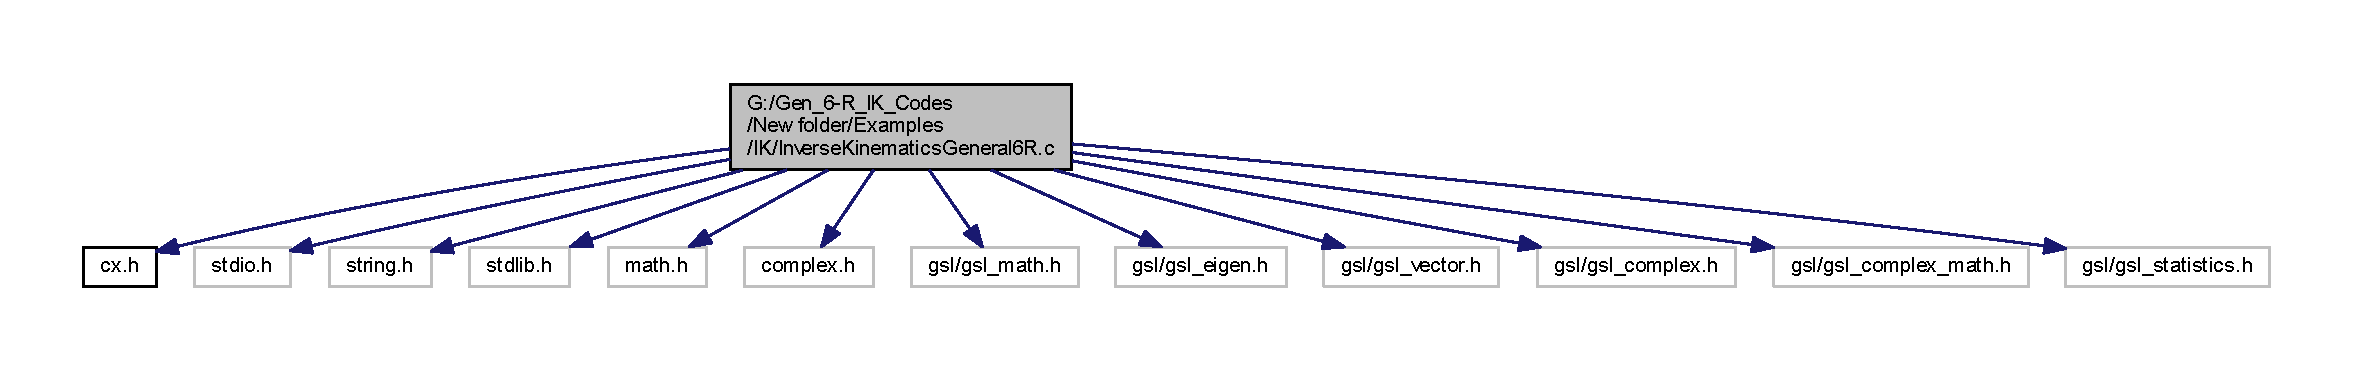
\includegraphics[width=350pt]{_inverse_kinematics_general6_r_8c__incl}
\end{center}
\end{figure}
\subsection*{Functions}
\begin{DoxyCompactItemize}
\item 
double \+\_\+\+Complex \hyperlink{_inverse_kinematics_general6_r_8c_a4d9425425b25a36edd0f0fdfd3e275e3}{user\+\_\+atan2\+\_\+c} (double \+\_\+\+Complex z1, double \+\_\+\+Complex z2)
\item 
struct \hyperlink{struct_solution}{Solution} \hyperlink{_inverse_kinematics_general6_r_8c_a86f312234822135a460f9bf458065774}{Inverse\+Kinematics\+General6R} (double dhmat\mbox{[}10\mbox{]}\mbox{[}10\mbox{]}, double eemat\mbox{[}10\mbox{]}\mbox{[}10\mbox{]})
\end{DoxyCompactItemize}


\subsection{Detailed Description}
The program is used to find the Inverse kinematics solutions for a general 6-\/R serial manipulator. 

\begin{DoxyDate}{Date}
September 30, 2017 
\end{DoxyDate}


\subsection{Function Documentation}
\mbox{\Hypertarget{_inverse_kinematics_general6_r_8c_a86f312234822135a460f9bf458065774}\label{_inverse_kinematics_general6_r_8c_a86f312234822135a460f9bf458065774}} 
\index{Inverse\+Kinematics\+General6\+R.\+c@{Inverse\+Kinematics\+General6\+R.\+c}!Inverse\+Kinematics\+General6R@{Inverse\+Kinematics\+General6R}}
\index{Inverse\+Kinematics\+General6R@{Inverse\+Kinematics\+General6R}!Inverse\+Kinematics\+General6\+R.\+c@{Inverse\+Kinematics\+General6\+R.\+c}}
\subsubsection{\texorpdfstring{Inverse\+Kinematics\+General6\+R()}{InverseKinematicsGeneral6R()}}
{\footnotesize\ttfamily struct \hyperlink{struct_solution}{Solution} Inverse\+Kinematics\+General6R (\begin{DoxyParamCaption}\item[{double}]{dhmat\mbox{[}10\mbox{]}\mbox{[}10\mbox{]},  }\item[{double}]{eemat\mbox{[}10\mbox{]}\mbox{[}10\mbox{]} }\end{DoxyParamCaption})}

Inverse\+Kinematics\+General6R\+: Function to compute the Inverse kinematics solutions for a general 6-\/R serial manipulator.


\begin{DoxyParams}{Parameters}
{\em dhmat} & A 2-\/D array containing the D-\/H parameters of the 6-\/R robot in cosideration. \\
\hline
{\em eemat} & A 2-\/D array containing the End-\/effector pose of the 6-\/R robot in consideration. The End-\/effector pose being described by the 3 x 3 rotation matix and 3x1 position vector.\\
\hline
\end{DoxyParams}
Further information about dhmat and eemat is given in the \textquotesingle{}Input files\textquotesingle{} section of the document \textquotesingle{}I\+K\+\_\+6\+R\+\_\+\+Program\+\_\+\+Documentation\textquotesingle{}.

Variables used\+: \tabulinesep=1mm
\begin{longtabu} spread 0pt [c]{*{2}{|X[-1]}|}
\hline
\rowcolor{\tableheadbgcolor}\textbf{ Variable }&\textbf{ Description  }\\\cline{1-2}
\endfirsthead
\hline
\endfoot
\hline
\rowcolor{\tableheadbgcolor}\textbf{ Variable }&\textbf{ Description  }\\\cline{1-2}
\endhead
rtod &Constant to convert angle in radians to angle in degrees. \\\cline{1-2}
lambda1 to lambda6 &cos(alpha1) to cos(alpha6), where alphai is from the D-\/H table. \\\cline{1-2}
mu1 to mu6 &sin(alpha1) to sin(alpha6), where alphai is from the D-\/H table. \\\cline{1-2}
vars &A 2-\/D array to store the D-\/H parameters and the End-\/effector pose of the 6-\/R robot in cosideration, to be used in other variables. \\\cline{1-2}
cmatx2 &The 12 x 12 coefficient matrix, \textquotesingle{}A\textquotesingle{}. \\\cline{1-2}
cmatx1 &The 12 x 12 coefficient matrix, \textquotesingle{}B\textquotesingle{}. \\\cline{1-2}
cmatx0 &The 12 x 12 coefficient matrix, \textquotesingle{}C\textquotesingle{}. The descriptions of A, B, and C is there in the following function. \\\cline{1-2}
cmatx01 to cmatx06 &The rows of the 6 x 9 submatrix used to form the 12 x 12 matrix, cmatx0. \\\cline{1-2}
cmatx11 to cmatx16 &The rows of the 6 x 9 submatrix used to form the 12 x 12 matrix, cmatx1. \\\cline{1-2}
cmatx21 to cmatx26 &The rows of the 6 x 9 submatrix used to form the 12 x 12 matrix, cmatx2. \\\cline{1-2}
i, j, l, m &counters used in the function. \\\cline{1-2}
angle &User-\/defined Structure type variable, \hyperlink{struct_solution}{Solution}. Its definition is there in the header file, \textquotesingle{}cx.\+h\textquotesingle{} \\\cline{1-2}
\end{longtabu}


\begin{DoxyReturn}{Returns}
angle 
\end{DoxyReturn}
The 12 x 12 matrix cmatx1 has also been formed in the same way as the matrix cmatx0. The rows of the 6 x 9 submatrix used in the formation of cmatx1 are cmatx11 to cmatx16. Each of the entries of these rows have been given a generic nomenclature of cx1ij, where i and j denotes the row position and column position of the entry in the submatrix, respectively.

Definition at line 79 of file Inverse\+Kinematics\+General6\+R.\+c.

Here is the caller graph for this function\+:\nopagebreak
\begin{figure}[H]
\begin{center}
\leavevmode
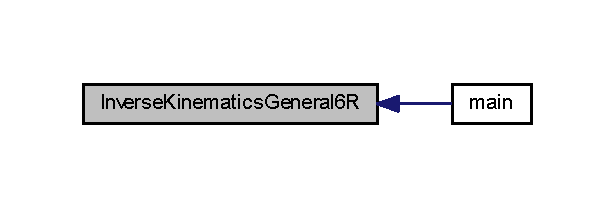
\includegraphics[width=295pt]{_inverse_kinematics_general6_r_8c_a86f312234822135a460f9bf458065774_icgraph}
\end{center}
\end{figure}
\mbox{\Hypertarget{_inverse_kinematics_general6_r_8c_a4d9425425b25a36edd0f0fdfd3e275e3}\label{_inverse_kinematics_general6_r_8c_a4d9425425b25a36edd0f0fdfd3e275e3}} 
\index{Inverse\+Kinematics\+General6\+R.\+c@{Inverse\+Kinematics\+General6\+R.\+c}!user\+\_\+atan2\+\_\+c@{user\+\_\+atan2\+\_\+c}}
\index{user\+\_\+atan2\+\_\+c@{user\+\_\+atan2\+\_\+c}!Inverse\+Kinematics\+General6\+R.\+c@{Inverse\+Kinematics\+General6\+R.\+c}}
\subsubsection{\texorpdfstring{user\+\_\+atan2\+\_\+c()}{user\_atan2\_c()}}
{\footnotesize\ttfamily double \+\_\+\+Complex user\+\_\+atan2\+\_\+c (\begin{DoxyParamCaption}\item[{double \+\_\+\+Complex}]{z1,  }\item[{double \+\_\+\+Complex}]{z2 }\end{DoxyParamCaption})}

user\+\_\+atan2\+\_\+c\+: gives the arc tangent of z2/z1, taking into account which quadrant the point (z1,z2) is in, where \textquotesingle{}z1\textquotesingle{} and \textquotesingle{}z2\textquotesingle{} are both complex nos.

Variables used\+: \tabulinesep=1mm
\begin{longtabu} spread 0pt [c]{*{2}{|X[-1]}|}
\hline
\rowcolor{\tableheadbgcolor}\textbf{ Variable }&\textbf{ Description  }\\\cline{1-2}
\endfirsthead
\hline
\endfoot
\hline
\rowcolor{\tableheadbgcolor}\textbf{ Variable }&\textbf{ Description  }\\\cline{1-2}
\endhead
z3 &Complex no. to store the output of the function, user\+\_\+atan2\+\_\+c. \\\cline{1-2}
\end{longtabu}
\begin{DoxyReturn}{Returns}
z3. 
\end{DoxyReturn}


Definition at line 37 of file Inverse\+Kinematics\+General6\+R.\+c.


\hypertarget{residue_8c}{}\section{G\+:/\+Gen\+\_\+6-\/\+R\+\_\+\+I\+K\+\_\+\+Codes/\+New folder/\+Examples/\+Residue/residue.c File Reference}
\label{residue_8c}\index{G\+:/\+Gen\+\_\+6-\/\+R\+\_\+\+I\+K\+\_\+\+Codes/\+New folder/\+Examples/\+Residue/residue.\+c@{G\+:/\+Gen\+\_\+6-\/\+R\+\_\+\+I\+K\+\_\+\+Codes/\+New folder/\+Examples/\+Residue/residue.\+c}}


This file is used to calculate residue1 to residue6 obtained by back-\/substituting the IK solutions into Eq.\+1-\/\+Eq.\+6 of the paper by Manocha and Canny and then taking the difference of the L.\+H.\+S. and R.\+H.\+S. of the aforementioned equations. 


{\ttfamily \#include $<$stdio.\+h$>$}\newline
{\ttfamily \#include $<$math.\+h$>$}\newline
{\ttfamily \#include $<$complex.\+h$>$}\newline
{\ttfamily \#include \char`\"{}cx.\+h\char`\"{}}\newline
Include dependency graph for residue.\+c\+:\nopagebreak
\begin{figure}[H]
\begin{center}
\leavevmode
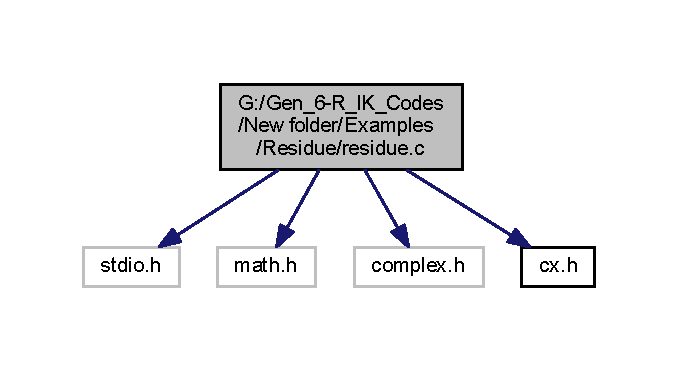
\includegraphics[width=326pt]{residue_8c__incl}
\end{center}
\end{figure}
\subsection*{Functions}
\begin{DoxyCompactItemize}
\item 
\mbox{\Hypertarget{residue_8c_a7b3454f7088b3001701b1102e54132df}\label{residue_8c_a7b3454f7088b3001701b1102e54132df}} 
struct \hyperlink{struct_residue}{Residue} {\bfseries residue} (double $\ast$coeff, double \+\_\+\+Complex $\ast$thlist)
\end{DoxyCompactItemize}


\subsection{Detailed Description}
This file is used to calculate residue1 to residue6 obtained by back-\/substituting the IK solutions into Eq.\+1-\/\+Eq.\+6 of the paper by Manocha and Canny and then taking the difference of the L.\+H.\+S. and R.\+H.\+S. of the aforementioned equations.


\hypertarget{theta1_8c}{}\section{G\+:/\+Gen\+\_\+6-\/\+R\+\_\+\+I\+K\+\_\+\+Codes/\+New folder/\+Examples/\+Theta/theta1.c File Reference}
\label{theta1_8c}\index{G\+:/\+Gen\+\_\+6-\/\+R\+\_\+\+I\+K\+\_\+\+Codes/\+New folder/\+Examples/\+Theta/theta1.\+c@{G\+:/\+Gen\+\_\+6-\/\+R\+\_\+\+I\+K\+\_\+\+Codes/\+New folder/\+Examples/\+Theta/theta1.\+c}}


This file is used to calculate the value of theta1 with the values of theta3, theta4, theta5, and the D-\/H parameters as input. 


{\ttfamily \#include $<$stdio.\+h$>$}\newline
{\ttfamily \#include $<$math.\+h$>$}\newline
{\ttfamily \#include $<$complex.\+h$>$}\newline
{\ttfamily \#include \char`\"{}cx.\+h\char`\"{}}\newline
Include dependency graph for theta1.\+c\+:\nopagebreak
\begin{figure}[H]
\begin{center}
\leavevmode
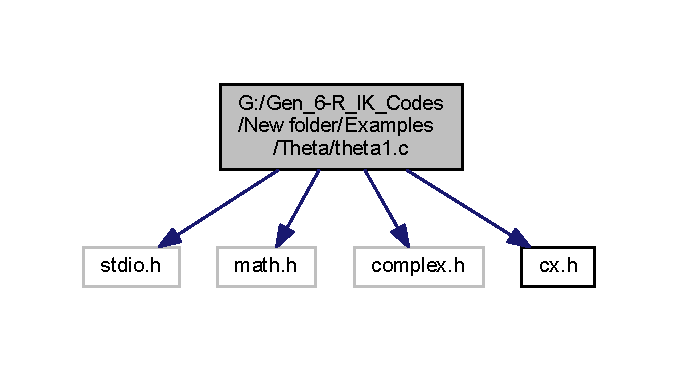
\includegraphics[width=326pt]{theta1_8c__incl}
\end{center}
\end{figure}
\subsection*{Functions}
\begin{DoxyCompactItemize}
\item 
\mbox{\Hypertarget{theta1_8c_a4596f8af579fecde1bbb65f7f2927bac}\label{theta1_8c_a4596f8af579fecde1bbb65f7f2927bac}} 
struct \hyperlink{struct_theta}{Theta} {\bfseries theta1} (double $\ast$coeff, double \+\_\+\+Complex $\ast$thlist)
\end{DoxyCompactItemize}


\subsection{Detailed Description}
This file is used to calculate the value of theta1 with the values of theta3, theta4, theta5, and the D-\/H parameters as input.


\hypertarget{theta2_8c}{}\section{G\+:/\+Gen\+\_\+6-\/\+R\+\_\+\+I\+K\+\_\+\+Codes/\+New folder/\+Examples/\+Theta/theta2.c File Reference}
\label{theta2_8c}\index{G\+:/\+Gen\+\_\+6-\/\+R\+\_\+\+I\+K\+\_\+\+Codes/\+New folder/\+Examples/\+Theta/theta2.\+c@{G\+:/\+Gen\+\_\+6-\/\+R\+\_\+\+I\+K\+\_\+\+Codes/\+New folder/\+Examples/\+Theta/theta2.\+c}}


This file is used to calculate the value of theta2 with the values of theta1, theta3, theta4, theta5, and the D-\/H parameters as input. 


{\ttfamily \#include $<$stdio.\+h$>$}\newline
{\ttfamily \#include $<$math.\+h$>$}\newline
{\ttfamily \#include $<$complex.\+h$>$}\newline
{\ttfamily \#include \char`\"{}cx.\+h\char`\"{}}\newline
Include dependency graph for theta2.\+c\+:\nopagebreak
\begin{figure}[H]
\begin{center}
\leavevmode
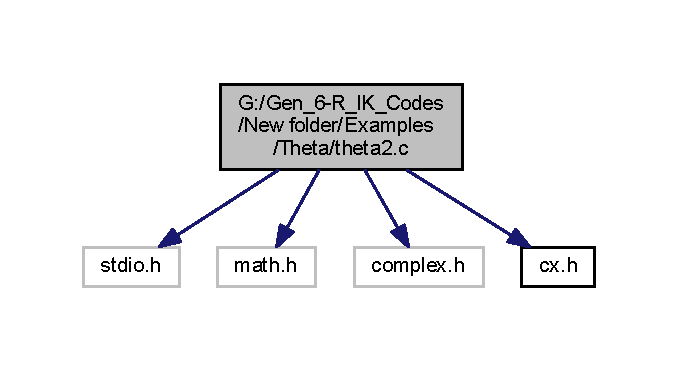
\includegraphics[width=326pt]{theta2_8c__incl}
\end{center}
\end{figure}
\subsection*{Functions}
\begin{DoxyCompactItemize}
\item 
\mbox{\Hypertarget{theta2_8c_a8bc4e7c2def044bafa4c187f708576f3}\label{theta2_8c_a8bc4e7c2def044bafa4c187f708576f3}} 
struct \hyperlink{struct_theta}{Theta} {\bfseries theta2} (double $\ast$coeff, double \+\_\+\+Complex $\ast$thlist)
\end{DoxyCompactItemize}


\subsection{Detailed Description}
This file is used to calculate the value of theta2 with the values of theta1, theta3, theta4, theta5, and the D-\/H parameters as input.


\hypertarget{theta6_8c}{}\section{G\+:/\+Gen\+\_\+6-\/\+R\+\_\+\+I\+K\+\_\+\+Codes/\+New folder/\+Examples/\+Theta/theta6.c File Reference}
\label{theta6_8c}\index{G\+:/\+Gen\+\_\+6-\/\+R\+\_\+\+I\+K\+\_\+\+Codes/\+New folder/\+Examples/\+Theta/theta6.\+c@{G\+:/\+Gen\+\_\+6-\/\+R\+\_\+\+I\+K\+\_\+\+Codes/\+New folder/\+Examples/\+Theta/theta6.\+c}}


This file is used to calculate the value of theta6 with the values of theta1, theta2, theta3, theta4, theta5, and the D-\/H parameters as input. 


{\ttfamily \#include $<$stdio.\+h$>$}\newline
{\ttfamily \#include $<$math.\+h$>$}\newline
{\ttfamily \#include $<$complex.\+h$>$}\newline
{\ttfamily \#include \char`\"{}cx.\+h\char`\"{}}\newline
Include dependency graph for theta6.\+c\+:\nopagebreak
\begin{figure}[H]
\begin{center}
\leavevmode
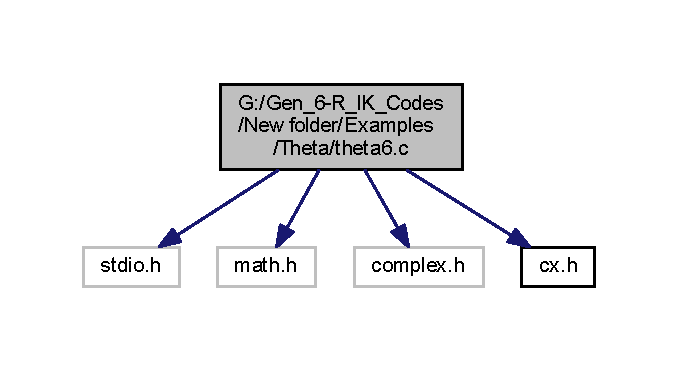
\includegraphics[width=326pt]{theta6_8c__incl}
\end{center}
\end{figure}
\subsection*{Functions}
\begin{DoxyCompactItemize}
\item 
\mbox{\Hypertarget{theta6_8c_affe129f4dc2f5c664559f4b0e426fb6c}\label{theta6_8c_affe129f4dc2f5c664559f4b0e426fb6c}} 
struct \hyperlink{struct_theta}{Theta} {\bfseries theta6} (double $\ast$coeff, double \+\_\+\+Complex $\ast$thlist)
\end{DoxyCompactItemize}


\subsection{Detailed Description}
This file is used to calculate the value of theta6 with the values of theta1, theta2, theta3, theta4, theta5, and the D-\/H parameters as input.


%--- End generated contents ---

% Index
\backmatter
\newpage
\phantomsection
\clearemptydoublepage
\addcontentsline{toc}{chapter}{Index}
\printindex

\end{document}
